% !TeX spellcheck = de_DE_frami
\section{Methodology}
\label{sec:methodology}
	
	\subsection{Measured Data}
	\label{ssec:measured-data}
	
		As a ...
		The reflectance $\varrho(\lambda)$ of a sample at a wavelength $\lambda \in \Lambda$ is recorded as
		\[
			-\lg \varrho(\lambda) = -\frac{\ln \varrho(\lambda)}{\ln 10}
		\]
		Figure \ref{fig:soil-spec-rnd} shows six randomly chosen soil spectra in a diagram.
		\begin{figure*}
			\centering
			% GNUPLOT: LaTeX picture with Postscript
\begingroup
  \makeatletter
  \providecommand\color[2][]{%
    \GenericError{(gnuplot) \space\space\space\@spaces}{%
      Package color not loaded in conjunction with
      terminal option `colourtext'%
    }{See the gnuplot documentation for explanation.%
    }{Either use 'blacktext' in gnuplot or load the package
      color.sty in LaTeX.}%
    \renewcommand\color[2][]{}%
  }%
  \providecommand\includegraphics[2][]{%
    \GenericError{(gnuplot) \space\space\space\@spaces}{%
      Package graphicx or graphics not loaded%
    }{See the gnuplot documentation for explanation.%
    }{The gnuplot epslatex terminal needs graphicx.sty or graphics.sty.}%
    \renewcommand\includegraphics[2][]{}%
  }%
  \providecommand\rotatebox[2]{#2}%
  \@ifundefined{ifGPcolor}{%
    \newif\ifGPcolor
    \GPcolorfalse
  }{}%
  \@ifundefined{ifGPblacktext}{%
    \newif\ifGPblacktext
    \GPblacktexttrue
  }{}%
  % define a \g@addto@macro without @ in the name:
  \let\gplgaddtomacro\g@addto@macro
  % define empty templates for all commands taking text:
  \gdef\gplbacktext{}%
  \gdef\gplfronttext{}%
  \makeatother
  \ifGPblacktext
    % no textcolor at all
    \def\colorrgb#1{}%
    \def\colorgray#1{}%
  \else
    % gray or color?
    \ifGPcolor
      \def\colorrgb#1{\color[rgb]{#1}}%
      \def\colorgray#1{\color[gray]{#1}}%
      \expandafter\def\csname LTw\endcsname{\color{white}}%
      \expandafter\def\csname LTb\endcsname{\color{black}}%
      \expandafter\def\csname LTa\endcsname{\color{black}}%
      \expandafter\def\csname LT0\endcsname{\color[rgb]{1,0,0}}%
      \expandafter\def\csname LT1\endcsname{\color[rgb]{0,1,0}}%
      \expandafter\def\csname LT2\endcsname{\color[rgb]{0,0,1}}%
      \expandafter\def\csname LT3\endcsname{\color[rgb]{1,0,1}}%
      \expandafter\def\csname LT4\endcsname{\color[rgb]{0,1,1}}%
      \expandafter\def\csname LT5\endcsname{\color[rgb]{1,1,0}}%
      \expandafter\def\csname LT6\endcsname{\color[rgb]{0,0,0}}%
      \expandafter\def\csname LT7\endcsname{\color[rgb]{1,0.3,0}}%
      \expandafter\def\csname LT8\endcsname{\color[rgb]{0.5,0.5,0.5}}%
    \else
      % gray
      \def\colorrgb#1{\color{black}}%
      \def\colorgray#1{\color[gray]{#1}}%
      \expandafter\def\csname LTw\endcsname{\color{white}}%
      \expandafter\def\csname LTb\endcsname{\color{black}}%
      \expandafter\def\csname LTa\endcsname{\color{black}}%
      \expandafter\def\csname LT0\endcsname{\color{black}}%
      \expandafter\def\csname LT1\endcsname{\color{black}}%
      \expandafter\def\csname LT2\endcsname{\color{black}}%
      \expandafter\def\csname LT3\endcsname{\color{black}}%
      \expandafter\def\csname LT4\endcsname{\color{black}}%
      \expandafter\def\csname LT5\endcsname{\color{black}}%
      \expandafter\def\csname LT6\endcsname{\color{black}}%
      \expandafter\def\csname LT7\endcsname{\color{black}}%
      \expandafter\def\csname LT8\endcsname{\color{black}}%
    \fi
  \fi
  \setlength{\unitlength}{0.0500bp}%
  \begin{picture}(7936.00,3400.00)%
    \gplgaddtomacro\gplbacktext{%
      \csname LTb\endcsname%
      \put(1078,704){\makebox(0,0)[r]{\strut{} 0.3}}%
      \csname LTb\endcsname%
      \put(1078,1190){\makebox(0,0)[r]{\strut{} 0.35}}%
      \csname LTb\endcsname%
      \put(1078,1676){\makebox(0,0)[r]{\strut{} 0.4}}%
      \csname LTb\endcsname%
      \put(1078,2163){\makebox(0,0)[r]{\strut{} 0.45}}%
      \csname LTb\endcsname%
      \put(1078,2649){\makebox(0,0)[r]{\strut{} 0.5}}%
      \csname LTb\endcsname%
      \put(1078,3135){\makebox(0,0)[r]{\strut{} 0.55}}%
      \csname LTb\endcsname%
      \put(1353,484){\makebox(0,0){\strut{} 1400}}%
      \csname LTb\endcsname%
      \put(2304,484){\makebox(0,0){\strut{} 1600}}%
      \csname LTb\endcsname%
      \put(3256,484){\makebox(0,0){\strut{} 1800}}%
      \csname LTb\endcsname%
      \put(4208,484){\makebox(0,0){\strut{} 2000}}%
      \csname LTb\endcsname%
      \put(5160,484){\makebox(0,0){\strut{} 2200}}%
      \csname LTb\endcsname%
      \put(6111,484){\makebox(0,0){\strut{} 2400}}%
      \csname LTb\endcsname%
      \put(7063,484){\makebox(0,0){\strut{} 2600}}%
      \put(176,1919){\rotatebox{-270}{\makebox(0,0){\strut{}$-\lg \varrho(\lambda)$}}}%
      \put(4374,154){\makebox(0,0){\strut{}$\lambda \ [\m{nm}]$}}%
    }%
    \gplgaddtomacro\gplfronttext{%
    }%
    \gplbacktext
    \put(0,0){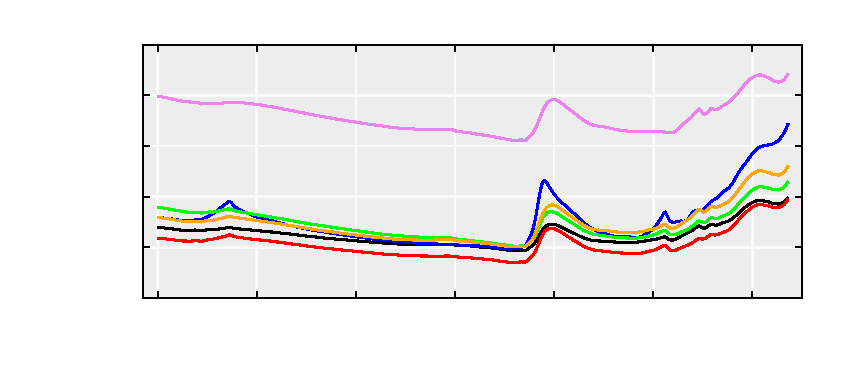
\includegraphics{gp/soil-spec-rnd}}%
    \gplfronttext
  \end{picture}%
\endgroup

			\caption{Six near infrared soil spectra of randomly chosen soil samples obtained from the data set, where $\lambda$ is the wavelength and $\rho(\lambda)$ the corresponding reflectance and each colour refers to one sample}
			\label{fig:soil-spec-rnd}
		\end{figure*}
		
	
	% subsection measured-data

	\subsection{Statistical Model}
	\label{ssec:statistical-model}
	
	
	

	
	% subsection statistical-model

	\subsection{Statistische Modellwahl im Falle von NIR-Spektroskopie}
	\label{ssec:mlr}
	Seien $Y\in \rm I\!R^{n}$ die Zielgröße eines statistischen Modellwahlverfahrens und $X \in \rm I\!R^{n \times d}$ die Matrix von $d$ Einflussparametern und $n$ Beobachtungen. 
	Zur Wahl einer geeigneten Menge von Einflussparametern $x_i$ auf die Zielgröße $y_i$  wird im klassischen linearen Modell die Modellwahl über eine hierarchische Aufstellung von linearen Modellen erriecht. Beginnend mit dem minimalen Modelle $E(Y_i) = \beta_0$ werden dem Modell nach und nach neue potenzielle Einflussparameter $x_{ik}$ hinzugefügt. Zu jedem dieser neuen $x_{ik}$ wird dann eine Teststatistik aufgestellt, die darauf hinweist, ob der gewählte Parameter wichtig ist ist oder nicht. Dabei ist die Nullhypothese, dass $x_{ik}$ keinen Einfluss auf die Zielgröße hat: $ H_0 = \beta_k = 0$ und wird abgelehnt, falls $H_1 = \beta_k \neq 0$ zutrifft. 
	Dies wird über die T-Teststatistik erreicht,  wobei für den Fall, dass $H_0$ richtig ist, gilt: $\frac{\hat{\beta_k}}{\sqrt{\sigma^2(X^TX)^{-1}_{kk}}} \sim t_{n-(k+1)}$.
	Mit diesem Modellwahlverfahren ergeben sich einige Schwierigkeiten, wobei die für unseren Fall besonders schwerwiegenden herausgehoben werden: In dieser Arbeit haben wir es mit einer großen Anzahl potenzieller Einflussvariablen auf dem Nah-Infrarotspekturm zu tun. A priori kann schwer eine inhaltliche Deutung vorgenommen werden, die gewisse Wellenlängen bevorzugt. Daher ist eine hierarchische Modellwahll mit wenigen, wohlüberlegten Einflussvariablen nicht möglich. Demnach muss in dieser Arbeit die Anzahl der möglichen Einflussgrößen stark erhöht werden und hier bekommen wir ein Problem mit der T-Teststatistik. Es ließen sich sehr viele unterschiedliche Kombinationen von Einflussgrößen aufstellen und in eine hierarchische Form bringen. Doch da wir bei der T-Teststatistik ein $\underline{zufälliges}$ Intervall konstruieren, gegen das unsere Hypothese getestet wird, ist die Wahrscheinlichkeit bei oft wiederholten Tests fälschlicherweise die Nullhypothese abzulehnen steigend mit Anzahl der Versuche. An ein automatisiertes Modellwahlverfahren, das in dieser Arbeit von Vorteil ist, ist also mittels des T-Tests nicht zu erreichen. (siehe Skript 11/2018)
	Stattdessen bietet sich eine Modellwahl basierend auf dem erwarteten Prognosefehler ("sum of prediction squared error", SPSE) an: 
	\begin{align}
		SPSE := E(\sum_{i=1}^{n} (Y_{i+n} - x_{i}^{(M)}\hat{\beta_i}^{((M)})^2)
	\end{align}
	
	Hierbei sind die Werte in $Y_{i+n}$ neue, potenzielle Beobachtungen zum Erwartungsvektor $x_i$ und $x_{i}^{(M)}\hat{\beta_i}^{((M)}$ ist sind die Prognosewerte aus dem Modell $M$. 
	Der Prognosefehler lässt sich in 3 Terme zerlegen: Einen irreduzierbaren Prognosefehler, der unabhängig von dem momentan betrachteten Modell ist, einen Biasterm, der die Abweichung des aktuellen Modells $M$ vom Prognosemodell als Summe der quadrierten Prognose-Verzerrungen anzeigt und einen Varianzterm, der die Ungenauigkeiten widerspiegelt, die sich aus der Schätzung von $(|M|+1)$ unbekannten Parametern ergibt. 
	Der SPSE lässt sich über unterschiedliche Wege berechnen / abschätzen, mithilfe neuer Beobachtungen (1), (wiederholter) Zerlegung der Ursprungsdaten in Test- und Trainingsdaten (2) oder mittels Schätzung basierend auf der Residuenquadratsumme ("residual squared sum", RSS), hier im Vergleich zu o.g. SPSE:
	 
	\begin{align}
	RSS^{(M)} := \sum_{i=1}^{n} E (Y_{i} - \hat{Y_i}^{(M)})^2
	\end{align}
	\begin{align}
	SPSE^{(M)} := \sum_{i=1}^{n} E (Y_{i+n} - \hat{Y_i}^{(M)})^2
	\end{align}

	Es kann gezeigt werden, dass RSS den Wert von SPSE systematisch unterschätzt, dass diese Unterschätzung jedoch behoben werden kann (siehe Skript 12/2018): 

	\begin{align}
	\mathchar"0362 SPSE^{(M)}} := RSS^{(M)} + 2 \tilde{\sigma}_{\underline{full}} ^2 (|M|+1)
	\end{align}
	
	
	
	% subsection mlr

	\subsection{Mallow's $C_{p}$}
	\label{ssec:mallows-C_p}
	

	\subsection{Simulated Annealing}
	\label{ssec:model-selec}
	
		We can 

	% subsection simulated-annealing
		
	\subsection{Model Validation}
	\label{ssec:model-validation}
	
	
	% subsection model-validation
	
	\subsection{Assessment by Simulation}
	\label{ssec:simulation}
	
		
		
	% subsection simulation
% section methodology